% 20200815
\documentclass[../thesis.tex]{subfiles} %% use packages & commands as this main file
\begin{document}

\subsection{The model}
The system is a set of ordinary differential equations (ODE).  It is a temperature-static system with two biological components (\phy\ and \bac) and three density state variables (organic carbon $C$, \phy\ biomass $P$ and \bac l biomass $B$; Fig.\ref{f:model}). \Phy\ and \bac\ receive carbon from different sources (\phy\ photosynthesize carbon dioxide from an external unlimited source; \bac\ consume organic carbon from the internal finite $C$ pool) but allocate carbon in the same way (respiration, leakage and biomass incorporation).  Some biomass from \phy/\bac\ die and become part of the $C$ pool.  Organic carbon in the environment can either be consumed by \bac, harvested out of the system or remained in the $C$ pool only.  There are four major assumptions:  \Rn{1}) homogeneous environmental conditions and light intensity (i.e. a system shaped as a thin panel); \Rn{2}) unlimited growth nutrient for \phy\ and \bac; \Rn{3}) constant system temperature; \Rn{4}) \bac\ have no carbon type preferences on consumption.  In short, living space for \phy\ is the only limiting factor.

The rate of change of state variables (carbon density per day, \dxdt) are the currencies in our equations.  The equations are composed of three state variables of carbon densities, four life history traits of \phy, four life history traits of \bac\ and one harvest rate parameter (Eq.\ref{eq:PBH}).

\begin{equation}\left\{\begin{array}{rl}
    C'(t) &= \ePR(1-\eP)\cdot\gP\cdot P +\aP\cdot P^2 +(\eBR(1-\eB)-1)\cdot\gB\cdot C\cdot B +\mB\cdot B -xC\\
    P'(t) &= \ePR\cdot\eP\cdot\gP\cdot P -\aP\cdot P^2\\
    B'(t) &= \eBR\cdot\eB\cdot\gB\cdot C\cdot B -\mB\cdot B
\end{array}\right.\label{eq:PBH}\end{equation}

In Eq.\ref{eq:PBH}, $C'(t)$, $P'(t)$ and $B'(t)$ are the rates of density change (\dxdt).  $\ePR$ is the fraction of non-respired carbon for $P$, $\eP$ is the fraction of carbon incorporated as $P$ biomass, $\eBR$ is the fraction of non-respired carbon for $B$ and $\eB$ is the fraction of carbon incorporated as $B$ biomass.  These four are ``fraction parameters”.  $\gP$ is the growth rate of $P$ (\dayU), $\aP$ is the intraspecific interference of $P$ (\denI), $\gB$ is the resource clearance rate of $B$  (\denI) and $\mB$ is the death rate of $B$ (\dayU).  These four are ``rate parameters”.  $x$ is the harvest rate (\dayU), which is the speed of carbon harvest from the $C$ pool in a continuous harvest system.  $x$ is set to zero in destructive harvest systems and the harvest interval $T$ (day) is the alternative parameter for the yield measurement.  The interval is defined as

\begin{equation*}
    T = x-1
    \label{eq:TvsX}
\end{equation*}

Values of equivalent $T$ and $x$ differ by 1 because the day of system establishment is day 0.  Continuous harvest starts on day 0 but destructive harvest starts on day 1.  Carbon yield from continuous harvest on the first day is equivalent to that by destructive harvest on the second day.

Daily yield in continuous harvest systems is defined as

\begin{equation}
    \text{daily yield} = x\cdot C
    \label{eq:yield}
\end{equation}

and the equivalent for destructive harvest is ``average yield", which is defined as

\begin{equation*}
    \text{average yield} = \dfrac{[\text{total carbon}]|_{T}-[\text{total carbon}]|_{0}}{T}
    \label{eq:avgYd}
\end{equation*}

\begin{figure}[H]
    \centering
    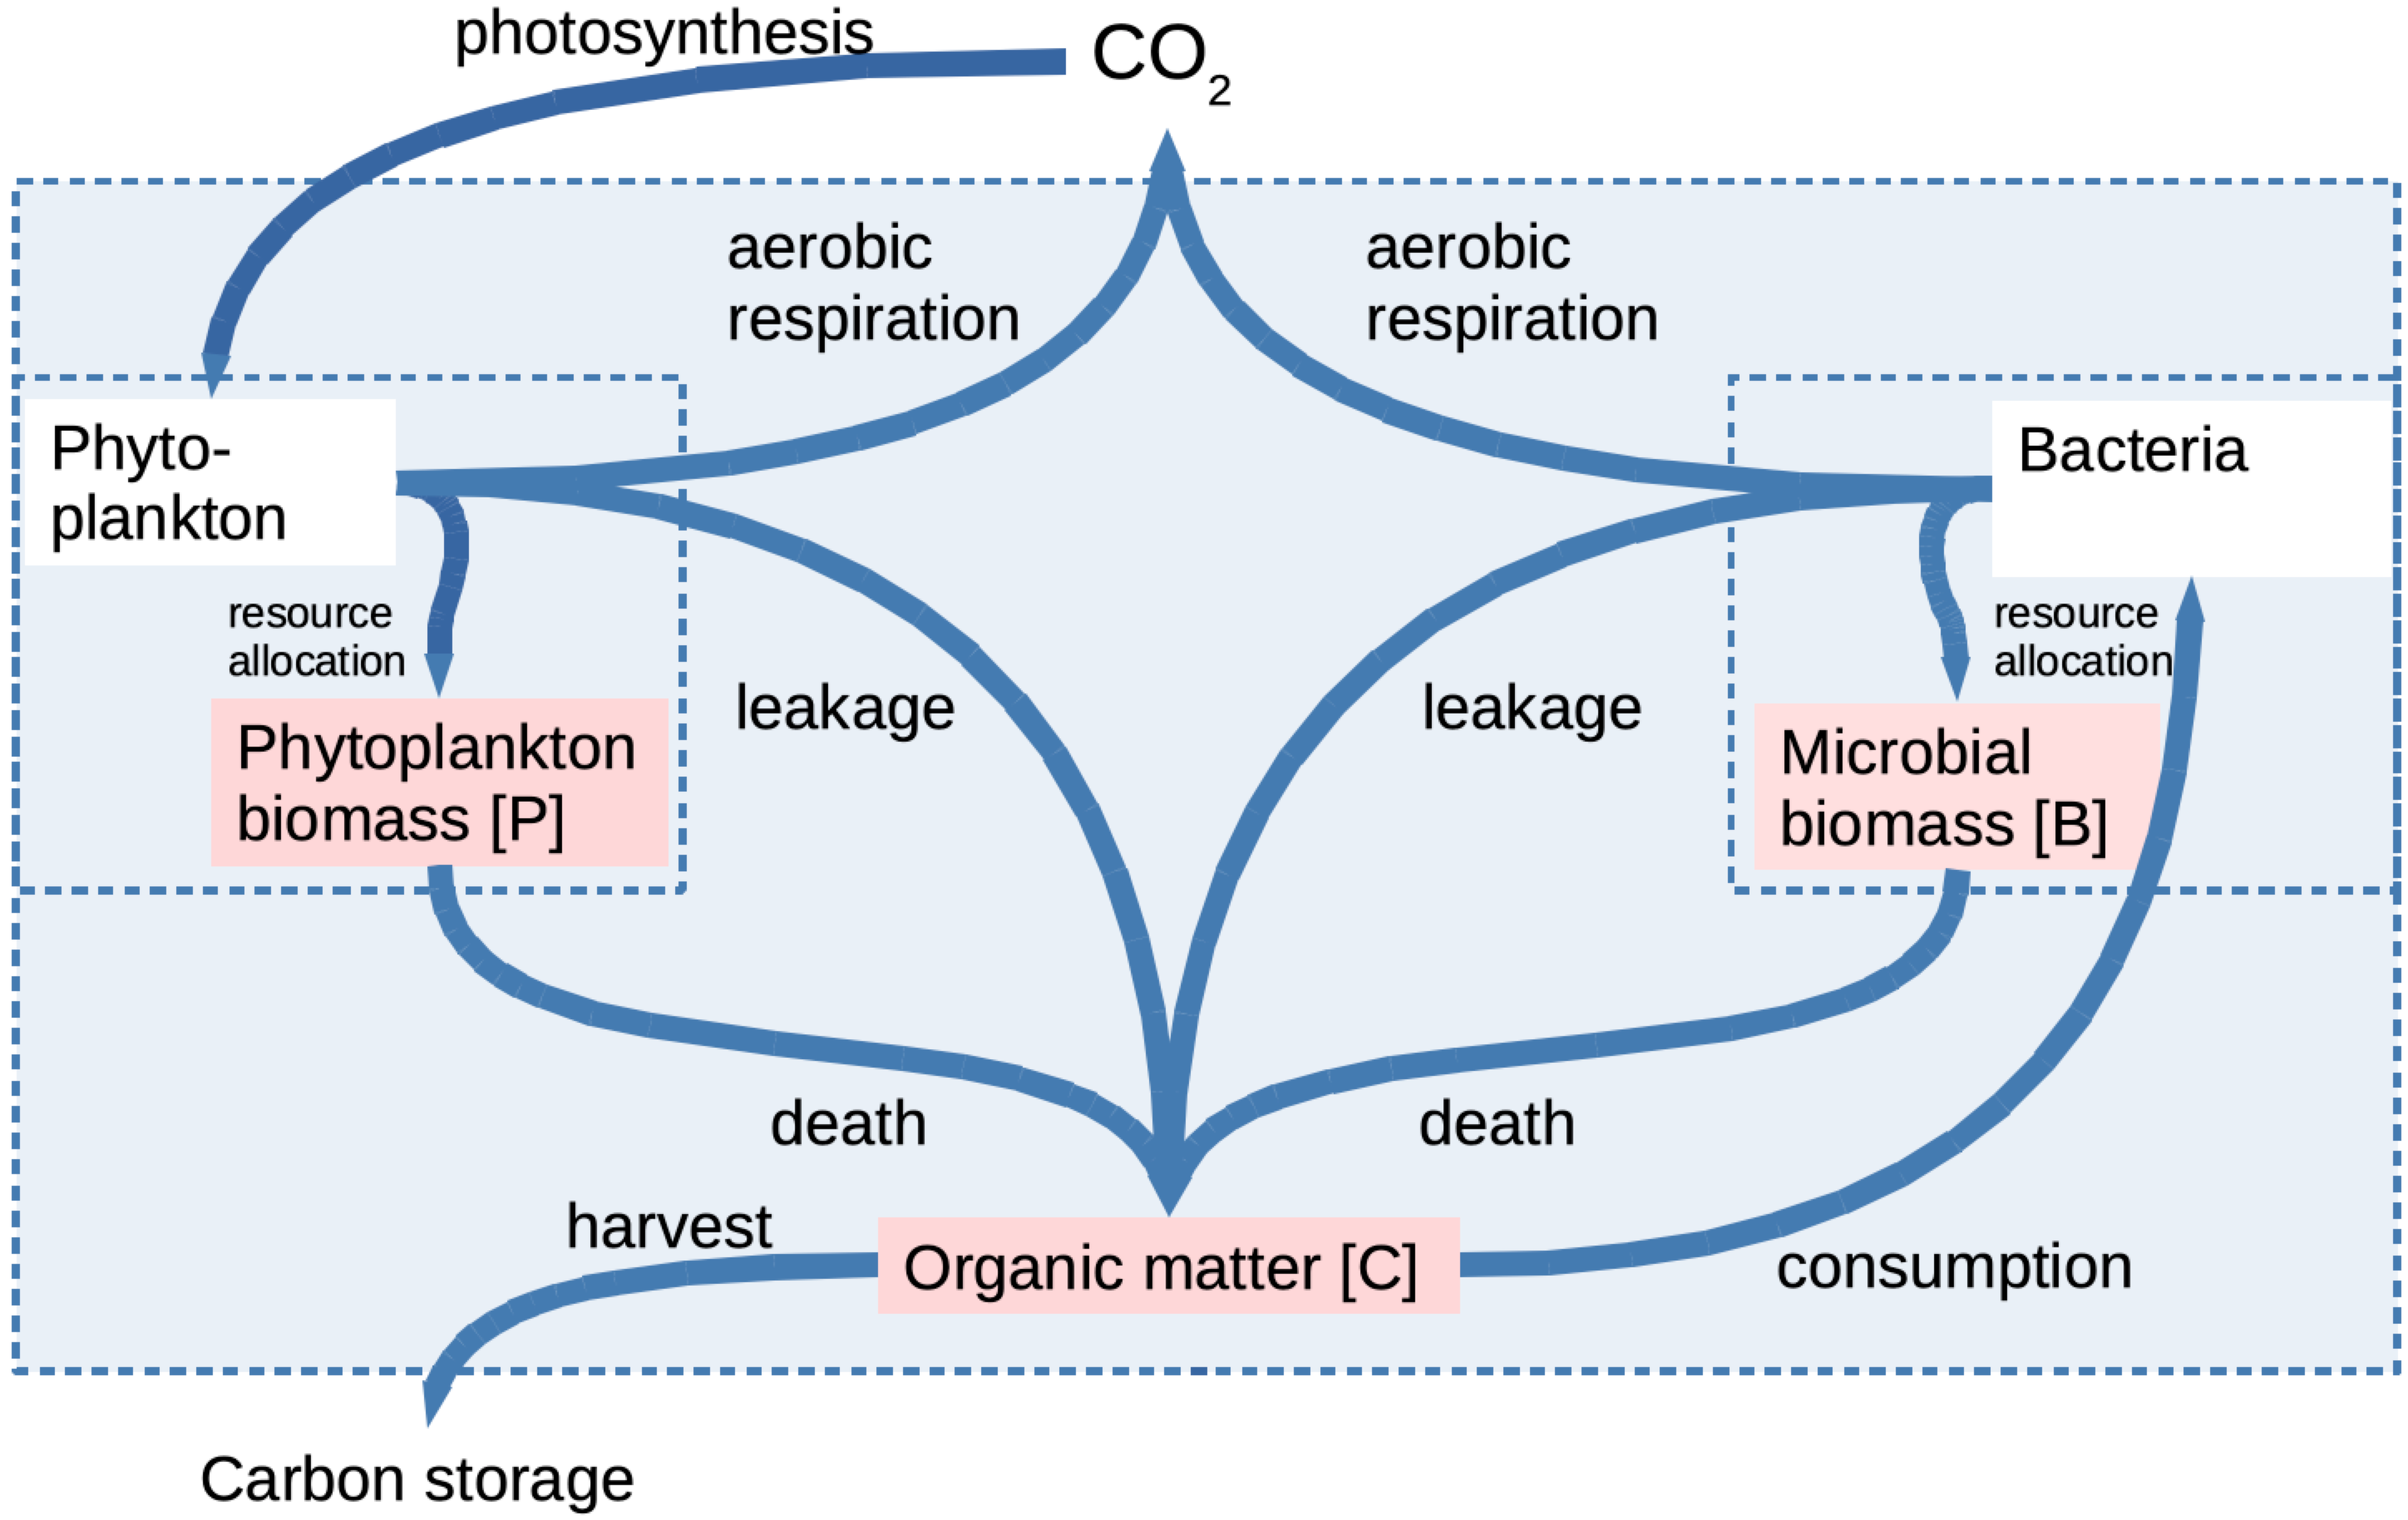
\includegraphics[width=.8\linewidth]{media/model.png}
    \caption[Model visualization]{The theoretical coexistence open system of \phy\ and \bac\ allows carbon exchange with external carbon dioxide source.  The dashed box is the defined boundary allowed matter exchange.  Blue arrows are the directions of carbon flow.  Pink boxes are the carbon pools (i.e. state variables).  White boxes are biochemical processes in indicated organisms.  These processes divert carbon from source to different carbon pools.}
    \label{f:model}
\end{figure}

Eq.\ref{eq:PBH} is a \pbs\ of $P$ and $B$ under continuous harvest (\PBH).  Three systems on $P$-only continuous harvest (\PoH), $P$ and $B$ destructive harvest (\PBN) and $P$-only destructive harvest (\PoN) were branched.

Continuous harvest \phy-only system (\PoH);
\begin{equation}\left\{\begin{array}{rl}
    C'(t) &= \ePR(1-\eP)\cdot\gP\cdot P +\aP\cdot P^2 -xC\\
    P'(t) &= \ePR\cdot\eP\cdot\gP\cdot P -\aP\cdot P^2
\end{array}\right.\label{eq:PoH}\end{equation}

Destructive harvest \pbs\ of $P$ and $B$ (\PBN); and
\begin{equation}\left\{\begin{array}{rl}
    C'(t) &= \ePR(1-\eP)\cdot\gP\cdot P +\aP\cdot P^2 +(\eBR(1-\eB)-1)\cdot\gB\cdot C\cdot B +\mB\cdot B\\
    P'(t) &= \ePR\cdot\eP\cdot\gP\cdot P -\aP\cdot P^2\\
    B'(t) &= \eBR\cdot\eB\cdot\gB\cdot C\cdot B -\mB\cdot B
\end{array}\right.\label{eq:PBN}\end{equation}

Destructive harvest \phy-only system (\PoN).
\begin{equation}\left\{\begin{array}{rl}
    C'(t) &= \ePR(1-\eP)\cdot\gP\cdot P +\aP\cdot P^2\\
    P'(t) &= \ePR\cdot\eP\cdot\gP\cdot P -\aP\cdot P^2
\end{array}\right.\label{eq:PoN}\end{equation}

Three biologically meaningful system stable states for continuous harvest systems are deduced using SymPy (v1.5.1) in python3 (v3.7.3) (Table \ref{t:eqm}).  Equilibrium 2 \& 3 are \PoH\ \& \PBH\ respectively. Equilibrium 1 was a default alternative stable state with no carbon in the system.  Destructive systems can only be investigated through integration because the analytical solutions are invalid; these solutions consisted with state variables only but not biological parameters.

\begin{table}[H]
    \centering
    \caption[Model equilibria]{Equilibria from the four variations of the proposed model (Eq.\ref{eq:PBH})}
    \begin{tabular}{cl|ccc}\hline
        equilibrium & scenario & $C$ & $P$ & $B$ (\PBH\ only) \\\hline
        1 & \PBH, \PoH & 0 & 0 & 0 \\
        2 & \PBH, \PoH & $\dfrac{\eP(\ePR\gP)^2}{\aP x}$ & $\dfrac{\ePR\eP\gP}{\aP}$ & 0 \\
        3 & \PBH & $\dfrac{\mB}{\eBR\eB\gB}$ & $\dfrac{\ePR\eP\gP}{\aP}$ & $\dfrac{(\ePR\gP)^2\eBR\eB\gB-\aP\mB x}{(1-\eBR)\aP\gB\mB}$ \\\hline
    \end{tabular}
    \label{t:eqm}
\end{table}

\subsection{Parameter space}
Data of the defined parameters in Eq. \ref{eq:PBH} was collected from literature (Supplementary sections 3-9).  Data was temperature-standardized to \temp\ to align with most data collected (Supplementary section 2).  Parameters less than five data points were called ``data deficient"; half of the parameters in Table \ref{t:ranges} ($\aP$, $\eBR$, $\eB$, $\mB$) were data deficient.  The widest percentage range in respective parameter groups (fraction or rate parameters) was inferred as the logical range for these data-deficient parameters.  The selection was based on the Metabolic Theory of Ecology \autocite{brown2004toward}, which suggested that similar body size organisms had similar metabolic rates.  \Phy\ and \bac\ had similar cell sizes as unicellular organisms.  Similar life history traits for \phy\ and \bac\ therefore would potentially share parameter ranges.  Ranges for each parameter was rooted around the mean of collected data bounded by the percentage range.  In each parameter range, 11 evenly-spaced sample values were selected.  The values formed a defined space of parameter combinations for model simulations.

\begin{table}[H]
    \centering
    \caption[Algebra variables]{Biological variables and corresponding ranges framing the parameter space}
    \begin{tabular}{cclll}\hline
        variable & unit & description & min & max \\\hline
        $N'(t)$ & \dxdt & rate of change of respective carbon pool {\tiny($N=C,P,B$)} & - & - \\
        $N$ & \den & carbon density for respective pool {\tiny($N=C,P,B$)} & - & - \\
        $\ePR$ & - & non-respired carbon fraction for $P$ & 0.08 & 0.87 \\
        $\eP$ & - & assimilated carbon fraction for $P$ & 0.40 & 1.00 \\
        $\gP$ & \dayU & growth rate of $P$ & 0.03 & 3.17 \\
        $\aP$ & \denI & intraspecific interference of $P$ & 0.02 & 1.52 \\
        $\eBR$ & - & non-respired carbon fraction for $B$ & 0.13 & 1.00 \\
        $\eB$ & - & assimilated carbon fraction for $B$ & 0.07 & 0.82 \\
        $\gB$ & \denI & clearance rate of $B$ & 0.10 & 3.50 \\
        $\mB$ & \dayU & death rate of $B$ & 0.01 & 0.63 \\
    \hline\end{tabular}
    \label{t:ranges}
\end{table}

\subsection{Scenario sampling}
A set of 5500 (11 sample values $\times$ 500 expected sample frequency) unique biological parameter combinations were randomly selected via a uniform prior with seed number ``20192020" in R (v4.0.2).  This Latin Hypercube Sampling (LHS) method was to ensure the widest parameter space covered with a limited sample size.  200 evenly-spaced harvest rates ($x$) ranged 1-19901 \dayU were applied on each set of biological parameter combinations on continuous harvest systems.  An equivalent harvest interval samples ($T$ = 0-19900 days, 200 evenly-spaced samples) were applied for each set of biological parameter combinations on destructive harvest systems.

\subsection{Model experiment}
Carbon densities of continuous harvest systems were analytically calculated by C-lang (compiler gcc v7.5.0) using equilibrium positions from Table \ref{t:eqm}. Yield in \PoH\ was independent from harvest rates as defined in Eq.\ref{eq:yield}.  Carbon densities of destructive harvest systems were numerically integrated by python3 (v3.7.3) SciPy (v1.2.3) ``odeint" function using Eq. \ref{eq:PBH}.  Initial densities for \PBN\ and \PoN\ were $C=P=B=1$ and $C=P=1$, $B=0$ \den\ respectively.  I also integrated destructive systems in a log-spaced time (range of $T$ = 0-100 days) to observe the system behaviour before reaching stability.

\subsection{Carbon yield analysis}
Feasible solutions were defined as non-negative abundances in all state variables for a scenario.  Unfeasible solutions were set as invalid data (NA) for observing yield distributions within feasibility limits.  All four systems had right-skewed carbon yield distributions with extremely high-valued outliers.  Pairwise Wilcox signed rank tests in R (v4.0.2) with bonferroni adjustment and no paired situations were therefore chosen for median comparisons between systems.  Destructive harvest system development was observed on a log-spaced time; \bac l effect on each harvest mode was examined through selected harvest parameters; and life history influences were deduced by observing the log carbon yield distribution across the parameter range of each trait.

\end{document}